% Circuit Simulator documentation
% Author: Michael Mekonnen

\documentclass[12pt]{amsart}

% Packages
\usepackage{hyperref}
\usepackage{graphicx}
\usepackage[T1]{fontenc}
\usepackage[utf8]{inputenc}
\usepackage{tikz}
\usetikzlibrary{shadows}

% Custom commands
% Title page utils
\newcommand{\HRule}{\rule{\linewidth}{0.5mm}}
% Graphics directory
\graphicspath{{./Images/}}
% Border specs
\setlength\fboxsep{0pt}
\setlength\fboxrule{0.5pt}
% Keystroke command
% Taken from: http://tex.stackexchange.com/questions/5226/keyboard-font-for-latex
\newcommand*\keystroke[1]{%
  \tikz[baseline=(key.base)]
    \node[%
      draw,
      fill=white,
      drop shadow={shadow xshift=0.25ex,shadow yshift=-0.25ex,fill=black,opacity=0.75},
      rectangle,
      rounded corners=2pt,
      inner sep=1pt,
      line width=0.5pt,
      font=\scriptsize\sffamily
    ](key) {#1\strut}
  ;
}

\title{Circuit Simulator Documentation [DRAFT]}

\begin{document}

\begin{titlepage}
\begin{center}

\textsc{\LARGE Massachusetts Institute of Technology}\\[1.5cm]

\textsc{\Large \bfseries 6.01}\\
\textsc{\Large Introduction to EECS I}\\[2.5cm]

\HRule \\[0.4cm]
{ \huge \bfseries Circuit Simulator Documentation [DRAFT]}\\[0.4cm]
\HRule \\[1.5cm]

\vfill

{\large \today}

\end{center}
\end{titlepage}

\maketitle

\tableofcontents

\section{Introduction}

\subsection{What is  Circuit Simulator?}

Circuit Simulator is a tool built to aid 6.01 students in the circuits module of the course. With this tool, students are able to draw schematics of circuits and analyze them. The most important feature of Circuit Simulator is that it can automatically produce protoboard layouts from circuit schematics.

\subsection{Outline}

Section \ref{sec:editting} will describe the editting capabilities of Circuit Simulator, and Section \ref{sec:analysis} will explore its analysis capabilities. Section \ref{sec:running} describes how to run Circuit Simulator.

Note that the descriptions below will provide keyboard shortcuts to some commands, but many of these shortcuts are not supported on Mac OS X.

TODO(mikemeko): change screenshots to Windows screenshots.

\section{Editting}
\label{sec:editting}

\subsection{Overview}

Figure \ref{fig:overview} gives an overview of the editor. A  circuit schematic can be drawn on a large drawing board, with components taken from the components palette. Once a schematic is completely drawn, it can be analyzed with quick button presses.

\begin{figure}
\fbox{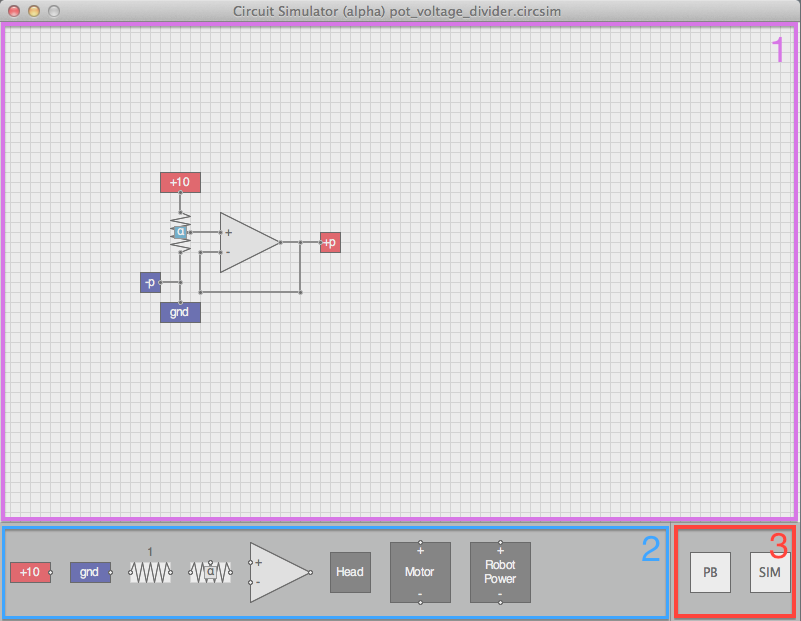
\includegraphics[width=\textwidth]{Editting_Overview.png}}
\caption{Box \textbf{1} (the drawing board) is the board where the schematic will be drawn. Box \textbf{2} (the components palette) is the area that contains all the components that can be added to the drawing board. Box \textbf{3} contains the analysis buttons.}
\label{fig:overview}
\end{figure}

\subsection{Adding, moving, and removing components}

To add a component to the drawing board, simply click the appropriate component in the components palette. Doing so adds an instance of the component to the drawing board.

To move a component on the drawing board, simply click and drag it. If the component is connected to other components via wires, the wires connected to the component will move as well. An alternative way of moving a component is clicking on the component and then using the arrow keys to move it.

To rotate a component on the board that is not connected to any wires, click on the component while holding \keystroke{Shift}.

To remove a component from the drawing board, click on the component while holding \keystroke{Ctrl} (or \keystroke{Control} on Mac OS X). Alternatively, click on the component and then press \keystroke{Delete} or \keystroke{Backspace}.

\subsection{Manipulating multiple components}

The Circuit Simulator editor allows manipulating multiple items at the same time. To do so, select a set of items using a selection rectangle by first clicking at an empty place on the board and dragging to extend the selection rectangle. Figure \ref{fig:selection} shows a set of selected items on the board. Once a set of items is selected, the user may move the items by using the arrow buttons, or delete the items by pressing \keystroke{Delete} or \keystroke{Backspace}.

\begin{figure}
\fbox{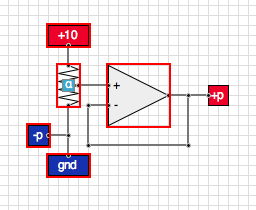
\includegraphics{Editting_Selection.png}}
\caption{Demonstration of a selected set of components on the drawing board.}
\label{fig:selection}
\end{figure}

\subsection{Connecting components}

Components may be connected via wires. To connect two components, click on one of the end-points of the first component and drag to reach an end-point of the second component. The editor attempts to draw a visually appealing connection between the components, but for closer user-control, the editor allows drawing floating wires.

\subsection{Undoing and redoing actions}

To Undo or Redo an action, click Edit $\rightarrow$ Undo (\keystroke{Ctrl}+\keystroke{z}) or Edit $\rightarrow$  Redo (\keystroke{Ctrl}+\keystroke{y}), respectively.

\subsection{Component descriptions}

\subsubsection{Power and Ground}

\fbox{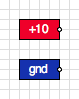
\includegraphics{Editting_Pwr_Gnd.png}}

Represent connections to the Power node (+10 volts) and Ground node.

\subsubsection{Robot Power}

\fbox{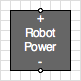
\includegraphics{Editting_Robot_Pwr}}

Represents connections to the Robot to draw Power (+10 volts) and Ground.

\subsubsection{Probes}

\fbox{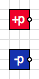
\includegraphics{Editting_Probes.png}}

Represent voltage probes used for analysis.

\subsubsection{Resistor}

\fbox{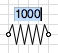
\includegraphics{Editting_Resistor.png}}

Represents resistors, of various resistances as set by the user.

\subsubsection{Pot}

\fbox{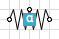
\includegraphics{Editting_Pot.png}}

Represents Potentiometers. The behavior of the pot is determined by the chosen signal file, which describes how the knob on the pot is being turned. A signal file for the pot can be chosen by right-clicking on the $\alpha$ sign.

\subsubsection{Op Amp}

\fbox{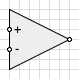
\includegraphics{Editting_Op_Amp.png}}

Represents Operational Amplifiers, clipped between +10 volts and ground.

\subsubsection{Motor}

\fbox{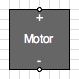
\includegraphics{Editting_Motor.png}}

Represents motors (via the motor connector).

\subsubsection{Head}

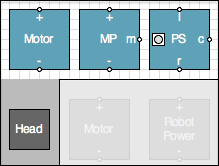
\includegraphics{Editting_Head.png}

Represents heads (connection to the robot via the head connector). A signal file indicating the distance and angle of the lamp can be chosen by righ-clicking on the lamp on the photosensor (PS) component.

\subsection{File management}

The Circuit Simulator editor allows saving files for later use. To save a file currently being edited, click File $\rightarrow$ Save (\keystroke{Ctrl} + \keystroke{s}). To open a saved file, click File $\rightarrow$ Open(\keystroke{Ctrl} + \keystroke{o}). To edit a new schematic, click File $\rightarrow$ New(\keystroke{Ctrl} + \keystroke{n}).

\section{Analysis}
\label{sec:analysis}

\subsection{Simulation}

Circuit Simulator outputs plots that describe the circuit. The independent variable for all plots is time.

If the probes are connected to the circuit, a plot will be output indicating the voltage difference between the probes.

For each pot, a plot will be given for its $\alpha$ signal.

Similarly, for each photosensor, plots will be given for its lamp angle and lamp distance signals.

For each motor, plots will be given for of the motor angle and the motor angular speed.

\subsection{Protoboard generation}

When the "PB" button is pressed, Circuit Simulator outputs a protoboard that corresponds to the drawn schematic. This is only done if the schematic is a reasonable circuit schematic. If Circuit Simulator fails to generate the protoboard, a message will be output saying so. Otherwise, a protoboard like the one shown in Figure \ref{fig:protoboard} will be output. This protoboard can be saved as a CMax layout by pressing File $\rightarrow$ Save as CMax file. This allows for later analysis with CMax.

\begin{figure}
\fbox{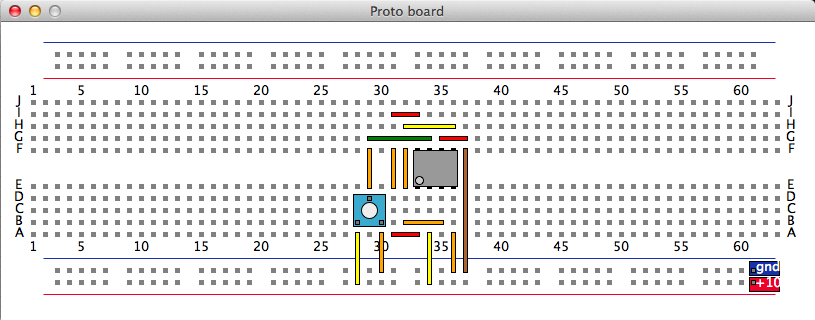
\includegraphics[width=\textwidth]{Output_Protoboard.png}}
\caption{Sample output protoboard for the schematic shown in Figures \ref{fig:overview} and \ref{fig:selection}.}
\label{fig:protoboard}
\end{figure}

\section{Running the Circuit Simulator}
\label{sec:running}
TODO(mikemeko): insert running instructions.

\end{document}
